\section{Background} \label{sec:background}

In this section, we will review evolvability from a biological perspective before shifting to a digital evolution perspective to discuss the relationship between the genotype-phenotype map and evolvability.
We will then touch on recently proposed equivalences between evolvability and machine learning.
Finally, we will put together a high-level understanding of the artificial neural network autoencoders AutoMap employs.

\subsection{Evolvability}
Although there is some inconsistency over the exact definition of evolvability in the literature, most thinking is consistent with the notion that evolvability stems from traits that facilitate the generation of \textit{novel} heritable phenotypic variation that is \textit{viable} \cite{tarapore2015evolvability}.
Let us examine a pair of biological examples of non-arbitrary phenotypic outcomes under mutation to build our intuition for evolvability.

A developmental constraint against certain non-viable phenotypic variation in  \textit{Drosophila melanogaster} was discovered through artificial selection experiments \cite{coyne1987lack, tuinstra1990lack}.
In these experiments,  researchers were able to successfully select for bilaterally symmetric phenotypic criteria, such as overall smaller eyes, but were unable to successfully select for bilaterally asymmetric phenotypic traits, such as different-sized eyes.
Tuinstra et al. hypothesize that the very nature of the developmental process constrains the phenotypic variation that can be observed in offspring, in this case curtailing the abundance of offspring that lack bilateral symmetry.
Specifically, they hypothesize that a lack of bilateral symmetry-breaking information during the embryological development of \textit{Drosophila} explains the negative result of artificial selection for bilaterally asymmetric phenotypic traits.
In this way, the distribution of phenotypic diversity in offspring is biased away from (likely non-viable) asymmetric variation.

In addition to qualities that constrain against non-viable mutational outcomes, biological organisms can possess qualities that facilitate significant heritable variation for a phenotypic trait.
Somatotropin, also known as growth hormone, is well known for its widespread anabolic effects on tissues throughout the body.
Mutations affecting the regulatory pathways that regulate somatotropin production and release, the receptors and cell signaling components that mediate cellular response to somatotropin, and the protein itself all provide avenues for significant heritable variation in body size \cite{devesa2016multiple}.
Dog breeds exhibit a range of body weights spanning nearly an entire order of magnitude.
Indeed, among certain groups of dogs, much of this variation can be explained by just six genes, several of which are associated with pathways somatotropin participates in \cite{rimbault2013derived}.
The presence of hormonal signaling pathways like those somatotropin participates in can be viewed as making a broad range of heritable phenotypic variation more readily realizable via mutation.

\subsection{Genotype-Phenotype Map and Evolvability}

In biological science, a distinction is drawn between an organism's genotype and phenotype.
Phenotype refers to an organism's observable characteristics (morphological, behavioral, physiological, chemical, etc.) that govern its interaction with the environment and ultimately determine its fitness.
Genotype refers the heritable information that influences the phenotype displayed by the individual, i.e. the organism's DNA.
Development is the process through which an organism's genotype shapes (but does not completely determine, due to environmental influence) its phenotype.
Under certain circumstances, it is useful to abstract development as a mathematical function that takes genetic information as its input and outputs phenotypic characteristics.
This mathematical function representing development is referred to as the genotype-phenotype map \cite{alberch1991genes}.

The nature of the genotype-phenotype map employed in an evolving system is thought to influence that system's evolvability \cite{pigliucci2010genotype}.
It is of theoretical interest to study genotype-phenotype maps and their relation to evolvability.
In digital evolution, it is also of practical interest to implement evolvable genotype-phenotype maps: more evolvable genotype-phenotype mappings enable more sophisticated digital evolution.
Let us discuss three theoretical constructs that are useful to understanding the relationship between the genotype-phenotype map and evolvability: latent evolvability, acquired evolvability, and innate evolvability.

The terms latent evolvability and acquired evolvability were introduced in \cite{reisinger2005towards} to discuss canalization, the ability of a population to bias the types of phenotypic variability generated among its offspring in order to exploit fitness biases specific to its environment.
Reisinger and Miikkulainen argue that canalization is a ``learned'' bias, developed over the course of evolution in response to selection pressure in a particular environment \cite{reisinger2005towards}.
Latent evolvability describes a genotype-phenotype map's potential to exhibit canalization while acquired evolvability describes actual canalization exhibited by an evolving population in response to a particular fitness environment.
I introduce the term innate evolvability to describe bias towards viable variation that is inherent to a genotype-phenotype map.
For example, Clune et al. identify bias towards phenotypic regularity, which in certain environments tends to be a useful trait, as an inherent quality of indirect genetic encoding \cite{clune2008generative}.

Innate, latent, and acquired evolvability each represent an opportunity for intervention by digital evolution practitioners in pursuit of evolvability.
Researchers can manually design an architecture for an evolving system (often inspired by properties and mechanisms of the developmental processes in nature) that exhibits strong innate \cite{clune2011performance} or latent \cite{reisinger2005towards} evolvability.
Indeed, hand-design of genotype-phenotype maps is ubiquitous in evolutionary computing \cite{wagner1996perspective}.
Genotype-phenotype mappings have been built that demonstrably exhibit latent \cite{reisinger2007acquiring} and innate \cite{stanley2009hypercube, clune2011performance} evolvability.
Such hand-designed genotype-phenotype mappings have been successfully employed to solve complex problems \cite{woolley2010evolving, cheney2013unshackling}.
Unfortunately, existing manually-designed genotype-phenotype mappings tend to be domain-specific --- a scheme useful for artificial neuroevolution, for example, likely is not useful in a linear genetic programming context.
In addition, sophisticated genotype-phenotype mappings --- particularly those extensively mimicking low-level aspects of embryological development --- can prove difficult to design and implement \cite[p 223]{downing2015intelligence}.

Selection techniques like evolvability selection \cite{mengistu2016evolvability}, modularly varying environments \cite{kashtan2005spontaneous}, the provision of a large number of niches for different tasks \cite{nguyen2015innovation} etc. can be employed to steer evolving populations towards regions of the genotype space that bestow acquired evolvability.
Although these approaches have been demonstrated successfully, they are inherently limited by the latent evolvability of the genotype-phenotype mapping that they are employed with \cite{reisinger2005towards}.

\subsection{Evolution and Learning}

In this article, we propose a fourth approach to achieve evolvability: directly learning an evolvable genotype-phenotype map from a training set of phenotypes harvested from local fitness peaks.
This idea is inspired by recent work explicitly framing evolution and evolvability in the context of learning theory \cite{kouvaris2017evolution, watson2016can}.
These authors point out that phenotypic variation generated under mutation and recombination is fundamentally shaped by an evolutionary history.
By this observation, they suggest an analogy between evolution and a machine learning system that exploits past experience to make informed decisions.
The key point is that undirected genetic variation can lead to structured phenotypic variation under a genotype-phenotype map that is shaped by evolutionary history \cite{watson2016can}.
Kourvais et al. specifically suggest that evolution might learn to generalize from past experience, essentially learning the structural regularities of phenotypes that were successful in the past and generating new phenotypes that are variations on that theme \cite{kouvaris2017evolution}.

\subsection{Autoencoder Neural Networks}

This AutoMap approach we propose to learn evolvable genotype-phenotype mappings relies on autoencoder neural networks.
We will take a brief detour to introduce these tools.

Autoencoders are artificial neural networks that are trained to regurgitate as output the input that they were provided.
Such networks are used to discover efficient lower-dimensional codings for datasets and, more recently, as method for generative modeling \cite{liou2014autoencoder, kingma2013auto}.
We will use two specific types of autoencoders: the bottlenecked autoencoder and the denoising autoencoder.

\begin{figure}
        \begin{subfigure}[b]{0.40\linewidth}
          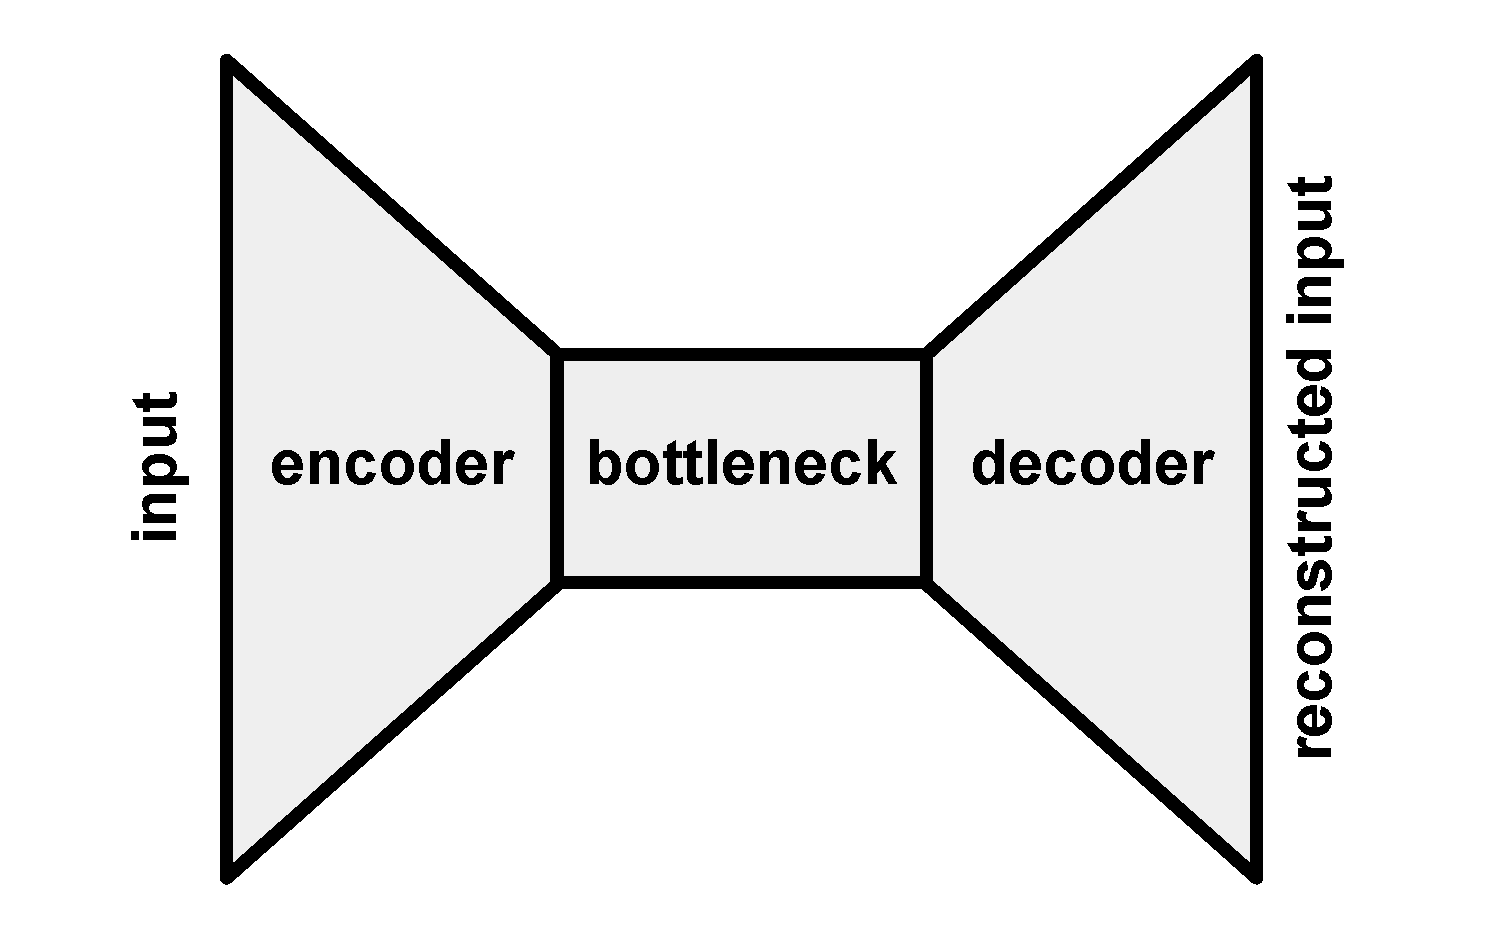
\includegraphics[width=\linewidth]{img/bottleneck}
          \subcaption{bottleneck autoencoder}
          \label{fig:bottleneck}
        \end{subfigure}%
        \begin{subfigure}[b]{0.40\linewidth}
          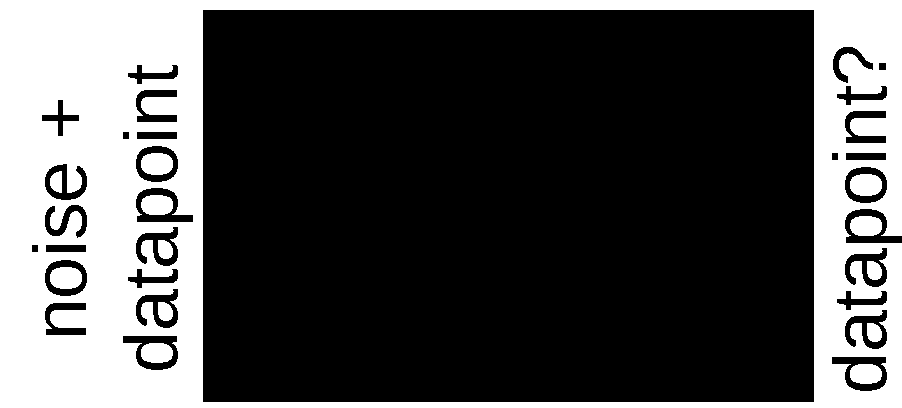
\includegraphics[width=\linewidth]{img/denoiser}
          \subcaption{denoising autoencoder}
          \label{fig:denoiser}
        \end{subfigure}%
        \caption{
          Schematics of bottlenecked a denoising autoencoders.
        }\label{fig:autoencoders}
\end{figure}


Figure \ref{fig:bottleneck} provides a schematic depiction of a bottleneck autoencoder.
This autoencoder has a small layer in the middle that information must pass through to reach the output.
Thus, the autoencoder is forced to learn a compact representation for the inputs it is trained with that can pass through the bottleneck.
The part of the autoencoder that precedes the bottleneck is called the encoder and the part that follows is called the decoder.

Figure \ref{fig:denoiser} provides a schematic depiction of a denoising autoencoder.
These autoencoders are trained to take noisy input and, from that noisy input, recover a signal in its original unadulterated form.
